\chapter{Etapa de Potencia, Sensado y Diseño del PCB}
\label{sec:potencia_pcb}

Las cuatro señales del secuenciador atacan finalmente la etapa de potencia encargada de conmutar la corriente de
ambas bobinas. En este capítulo revisamos el puente H doble, sus diodos de protección, el conector de retorno de
corriente y el trazado físico de la placa.

\section{Doble Puente H y Red de Protección Inductiva}
\label{sec:puente_h_diodos}

La etapa de salida emplea el integrado \texttt{IC1} (\texttt{L298N}, encapsulado Multiwatt-15), que reúne dos
puentes H independientes de hasta $46\V$ y $2\A$ continuos por canal. Recibe potencia de \texttt{VS} (pin 4),
$+5\V$ lógicos de \texttt{VSS} (pin 9) y masa en el pin 8 (\texttt{GND}).

El puente A toma \texttt{IN1} (pin 5) e \texttt{IN2} (pin 7) para manejar la fase A entre \texttt{OUT1} (pin 2) y
\texttt{OUT2} (pin 3), conectadas a \texttt{J4.1} y \texttt{J4.2}. El puente B toma \texttt{IN3} (pin 10) e
\texttt{IN4} (pin 12) para manejar la fase B entre \texttt{OUT3} (pin 13) y \texttt{OUT4} (pin 14) en
\texttt{J4.3} y \texttt{J4.4}. Ambos puentes se habilitan juntos mediante \texttt{ENABLE\_A} (pin 6) y
\texttt{ENABLE\_B} (pin 11).

Como sus salidas usan transistores bipolares, cada rama conductora presenta una caída de saturación combinada
($V_{CE\text{sat}(H)} + V_{CE\text{sat}(L)}$) de $3.7\V$ típicos a $2\A$ ($4.9\V$ máx.). Esa potencia disipada en
calor obliga a elegir una fuente \texttt{V+} acorde al motor y colocar disipador sobre la aleta metálica de
\texttt{IC1}.

Al invertir la corriente de una bobina o bajar \texttt{ENABLE}, la inductancia del devanado genera picos de
tensión $v_L = L\,\mathrm{d}i/\mathrm{d}t$ que pueden dañar el integrado. Para absorberlos instalamos ocho diodos
Schottky rápidos \texttt{D2}--\texttt{D9} (\texttt{1N5822}, $40\V$, $3\A$) dispuestos según la
figura~\ref{crkt.ej4:puente_diodos}.

\begin{figure}[!ht]
  \centering
  \begin{circuitikz}[american, scale=0.82, transform shape]
  % Bloque IC1 L298N
  \draw[thick, fill=orange!6] (-0.2,-4.3) rectangle (2.7,8.4);
  \node[align=center, font=\small\bfseries] at (1.25,7.8) {\texttt{IC1}\\L298N};

  % Salidas hacia J4 (espaciadas para evitar cruces con diodos)
  \draw (2.7,7.0) node[left, font=\scriptsize] {\texttt{OUT1} (2)} -- (9.6,7.0);
  \draw (2.7,4.2) node[left, font=\scriptsize] {\texttt{OUT2} (3)} -- (9.6,4.2);
  \draw (2.7,1.4) node[left, font=\scriptsize] {\texttt{OUT3} (13)} -- (9.6,1.4);
  \draw (2.7,-1.4) node[left, font=\scriptsize] {\texttt{OUT4} (14)} -- (9.6,-1.4);

  % Pines de sensado 1 y 15 unificados hacia J5 (por debajo de D9)
  \draw (2.7,-3.6) node[left, font=\scriptsize] {\texttt{SEN\_A} (1)} -- (3.4,-3.6);
  \draw (2.7,-4.0) node[left, font=\scriptsize] {\texttt{SEN\_B} (15)} -- (3.4,-4.0) -- (3.4,-3.6);
  \draw (3.4,-3.6) to[short, *-] (9.6,-3.6) to[short, -o] (9.6,-3.6)
    node[right, font=\scriptsize] {\texttt{J5.2 (SENSE\_A)}};
  \draw (9.6,-4.3) node[ground] {} to[short, -o] (9.6,-4.3)
    node[right, font=\scriptsize] {\texttt{J5.1 (GND)}};

  % Par D2/D3 en OUT1 (x = 4.5)
  \draw (4.5,7.0) to[sD*, l=$D_2$, *-] (4.5,8.4) node[above, font=\scriptsize] {\texttt{VS}};
  \draw (4.5,5.6) node[ground] {} to[sD*, l=$D_3$, -*] (4.5,7.0);

  % Par D4/D5 en OUT2 (x = 6.7)
  \draw (6.7,4.2) to[sD*, l=$D_4$, *-] (6.7,5.6) node[above, font=\scriptsize] {\texttt{VS}};
  \draw (6.7,2.8) node[ground] {} to[sD*, l=$D_5$, -*] (6.7,4.2);

  % Par D6/D7 en OUT3 (x = 4.5)
  \draw (4.5,1.4) to[sD*, l=$D_6$, *-] (4.5,2.8) node[above, font=\scriptsize] {\texttt{VS}};
  \draw (4.5,0.0) node[ground] {} to[sD*, l=$D_7$, -*] (4.5,1.4);

  % Par D8/D9 en OUT4 (x = 6.7)
  \draw (6.7,-1.4) to[sD*, l=$D_8$, *-] (6.7,0.0) node[above, font=\scriptsize] {\texttt{VS}};
  \draw (6.7,-2.8) node[ground] {} to[sD*, l=$D_9$, -*] (6.7,-1.4);

  % Etiquetas J4 y bobinas del motor paso a paso
  \node[above left, font=\scriptsize] at (9.6,7.0) {\texttt{J4.1}};
  \node[below left, font=\scriptsize] at (9.6,4.2) {\texttt{J4.2}};
  \node[above left, font=\scriptsize] at (9.6,1.4) {\texttt{J4.3}};
  \node[below left, font=\scriptsize] at (9.6,-1.4) {\texttt{J4.4}};

  \draw (9.6,7.0) to[L, l=Fase A, o-o] (9.6,4.2);
  \draw (9.6,1.4) to[L, l=Fase B, o-o] (9.6,-1.4);
\end{circuitikz}

  \caption{Etapa de salida del \texttt{L298N}, red de diodos Schottky y retorno de sensado en \texttt{J5}.}
  \label{crkt.ej4:puente_diodos}
\end{figure}

Cada terminal \texttt{OUT1}--\texttt{OUT4} queda protegido por dos diodos complementarios: los superiores
(\texttt{D2}, \texttt{D4}, \texttt{D6}, \texttt{D8}) derivan al bus \texttt{VS} (y a los capacitores \texttt{C1}
y \texttt{C5}) cualquier pulso por encima de $V_S + V_F$, mientras que los inferiores (\texttt{D3}, \texttt{D5},
\texttt{D7}, \texttt{D9}) conducen hacia \texttt{GND} cuando un nodo cae por debajo de $-V_F$. Se eligieron
diodos Schottky \texttt{1N5822} por su baja caída directa ($V_F \approx 0.45\V$ a $0.525\V$ entre $2\A$ y $3\A$)
y respuesta instantánea sin carga de recuperación inversa.

\section{Retorno de Corriente y Conexión para Sensado Externo}
\label{sec:sensado_corriente}

En el \texttt{L298N}, los emisores inferiores de ambos puentes salen al exterior por los pines
\texttt{CURRENT\_SENSING\_A} (pin 1) y \texttt{CURRENT\_SENSING\_B} (pin 15). En \texttt{ctrl\_pap}, los dos se
unen en la pista \texttt{SENSE\_A} hacia el pin 2 de \texttt{J5}, quedando \texttt{GND} en el pin 1.

Como toda la corriente del motor pasa por \texttt{J5} antes de volver a masa, la placa admite dos formas de
conexión:

\begin{enumerate}
  \item Integrada al CNC: \texttt{J5} se cablea hacia el módulo analógico de sensado externo, donde una
    resistencia derivadora hacia \texttt{GND} genera una tensión proporcional al consumo total de ambas fases para
    detectar topes o sobrecargas mecánicas.
  \item Prueba autónoma en banco: sin módulo de sensado conectado, resulta obligatorio colocar un puente o una
    resistencia entre los pines 1 y 2 de \texttt{J5}; si quedan abiertos, los puentes H no cierran circuito a
    masa y el motor no gira.
\end{enumerate}

\section{Diseño del Circuito Impreso y Lista de Materiales}
\label{sec:diseno_pcb}

La placa se diseñó en KiCad 10.0 en doble cara FR-4 de $1.6\,\unit{\milli\meter}$ con medidas exteriores de
$79.89\,\unit{\milli\meter} \times 74.08\,\unit{\milli\meter}$ ($5918.84\,\unit{\milli\meter\squared}$). Todos los
componentes utilizan montaje pasante sobre la cara superior para simplificar el armado manual y el reemplazo de
integrados. El esquemático eléctrico completo aparece en la figura~\ref{fig.ej4:esquematico_completo}.

\begin{figure}[!ht]
  \centering
  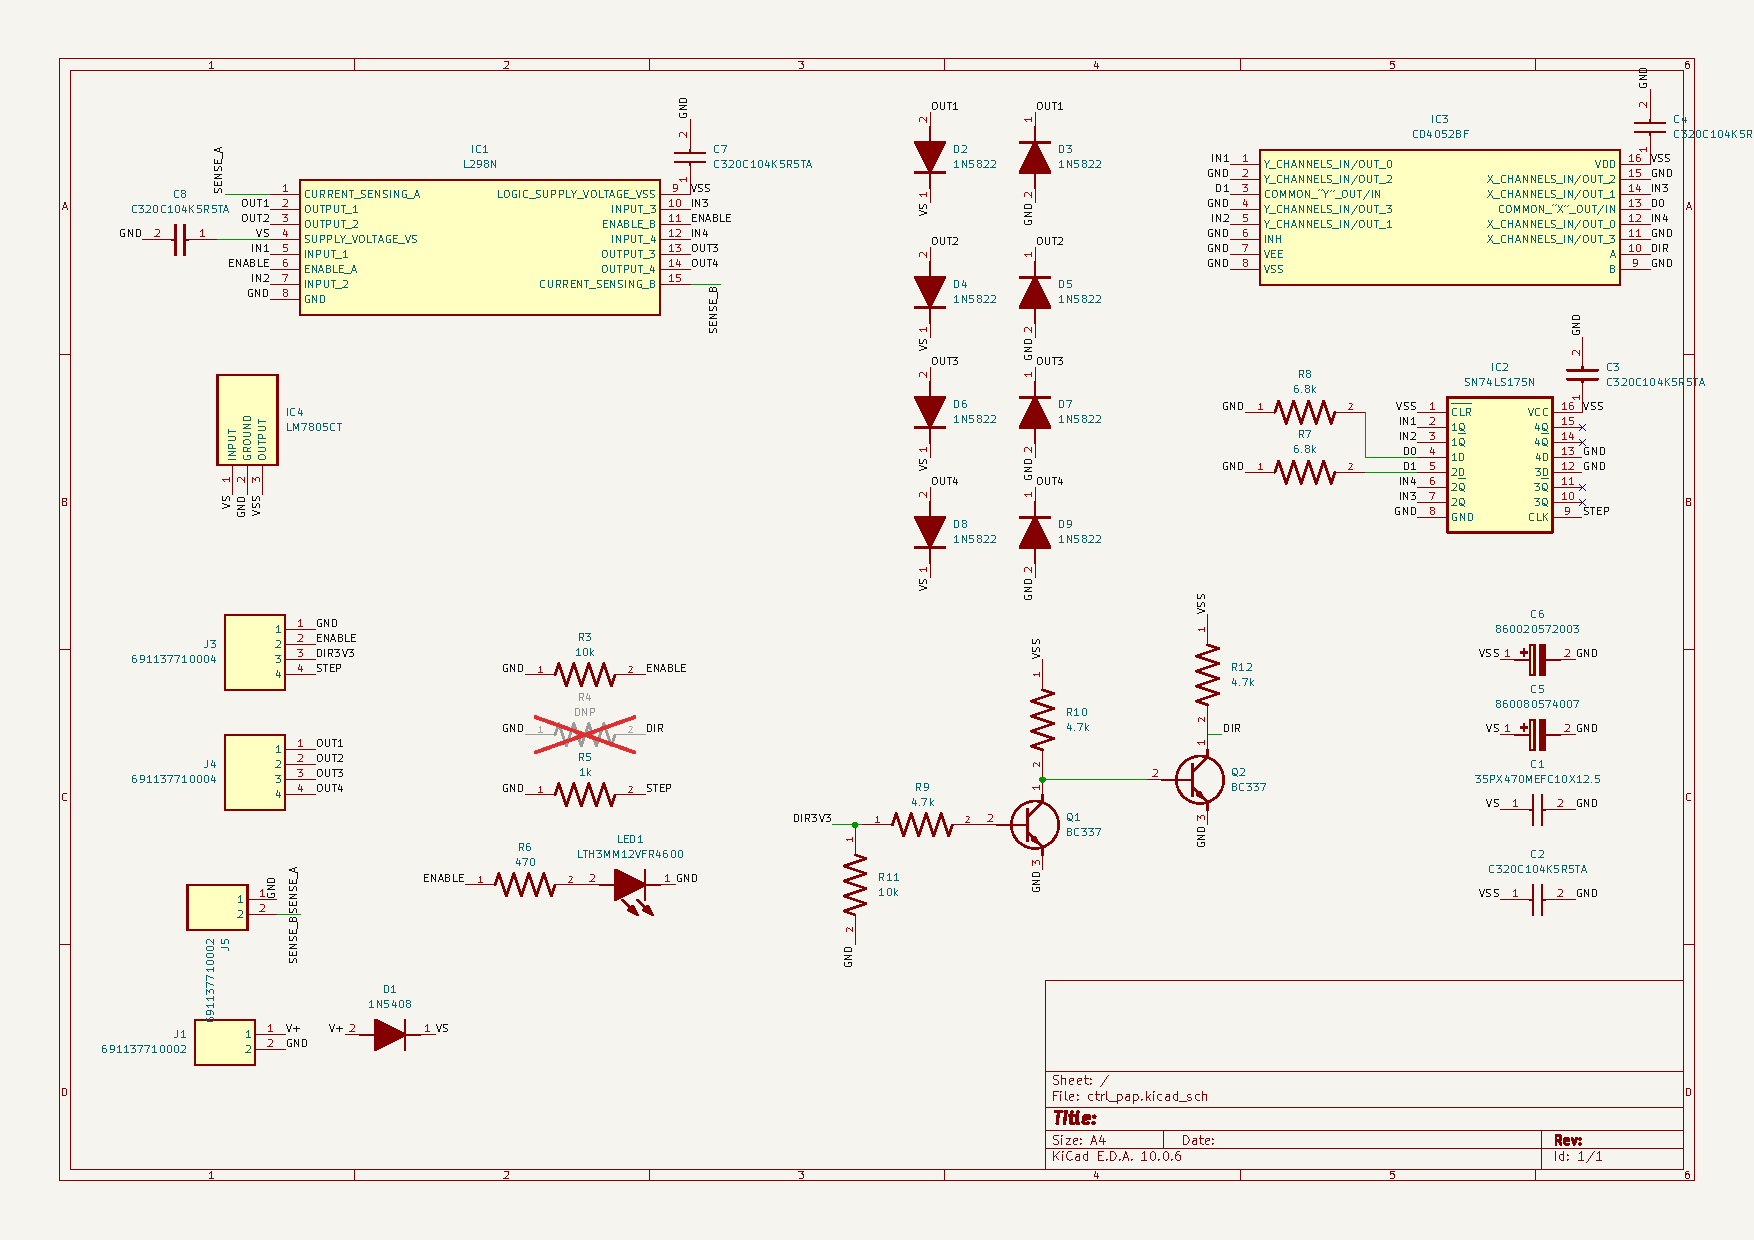
\includegraphics[width=\textwidth]{esquematico_ctrl_pap.pdf}
  \caption{Esquemático eléctrico completo de la placa controladora \texttt{ctrl\_pap}.}
  \label{fig.ej4:esquematico_completo}
\end{figure}

El ruteado mostrado en las vistas 3D de la figura~\ref{fig.ej4:vistas_pcb} sigue cuatro criterios simples:

\begin{itemize}
  \item Agrupación por etapa: arriba se ubican potencia y salidas (\texttt{IC1}, \texttt{D2}--\texttt{D9},
    \texttt{J4}); abajo a la izquierda entrada y regulación (\texttt{J1}, \texttt{D1}, \texttt{C1}, \texttt{C5},
    \texttt{IC4}, \texttt{J5}); en el centro la lógica (\texttt{IC2}, \texttt{IC3}); y a la derecha el control
    (\texttt{J3}, \texttt{Q1}, \texttt{Q2}, \texttt{LED1}).
  \item Ancho de pistas según corriente: señales digitales (\texttt{D0}, \texttt{D1}, \texttt{DIR}) en
    $0.7\,\unit{\milli\meter}$; salidas (\texttt{OUT1}--\texttt{OUT3}), \texttt{SENSE\_A} y \texttt{V+} en
    $1.0\,\unit{\milli\meter}$ ($1.3\,\unit{\milli\meter}$ en tramos de \texttt{OUT4} y \texttt{ENABLE}); y el bus
    \texttt{VS} en $1.5\,\unit{\milli\meter}$.
  \item Plano de masa inferior: la cara \texttt{B.Cu} cubre $5575.05\,\unit{\milli\meter\squared}$ con \texttt{GND},
    aislamiento mínimo de $0.2\,\unit{\milli\meter}$ y alivio térmico de $1.0\,\unit{\milli\meter}$ en pads.
  \item Montaje mecánico de \texttt{IC1}: su aleta metálica da al borde superior para fijar un disipador de
    aluminio sin estorbar otros componentes.
\end{itemize}

\begin{figure}[!ht]
  \centering
  \begin{subfigure}[t]{0.48\textwidth}
    \centering
    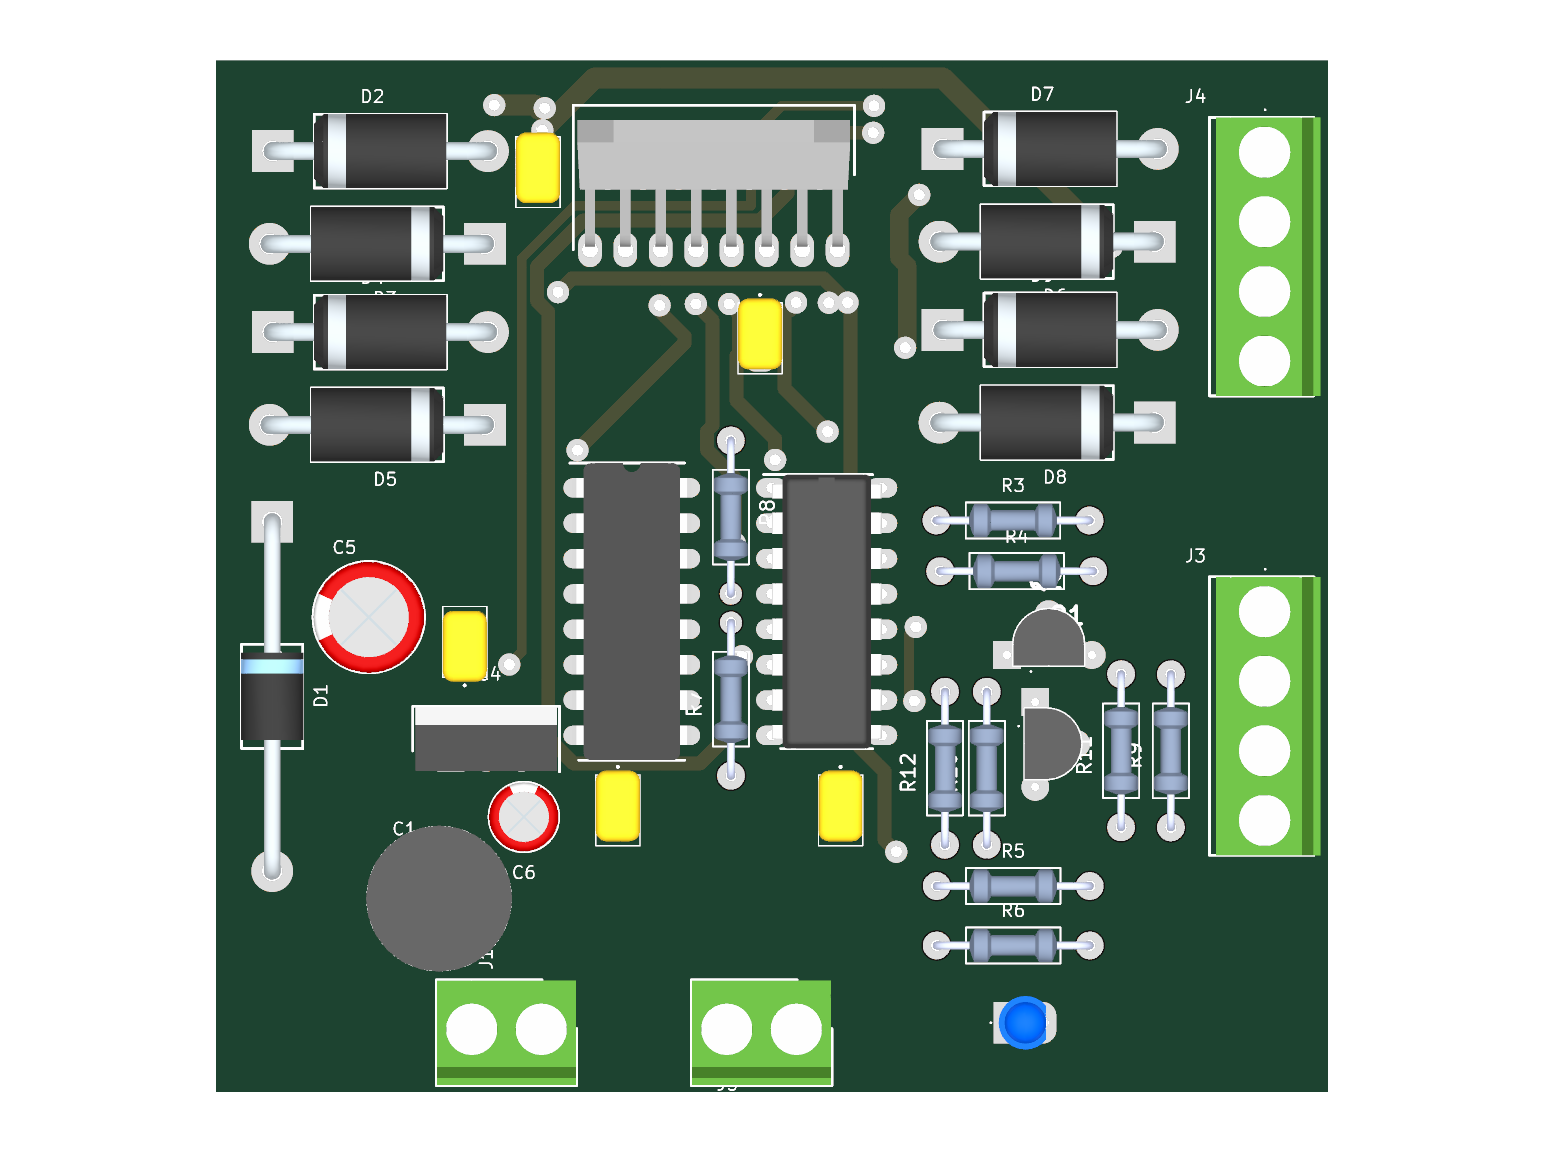
\includegraphics[width=\textwidth]{pcb_top.png}
    \caption{Vista superior de montaje de componentes.}
    \label{fig.ej4:pcb_top}
  \end{subfigure}
  \hfill
  \begin{subfigure}[t]{0.48\textwidth}
    \centering
    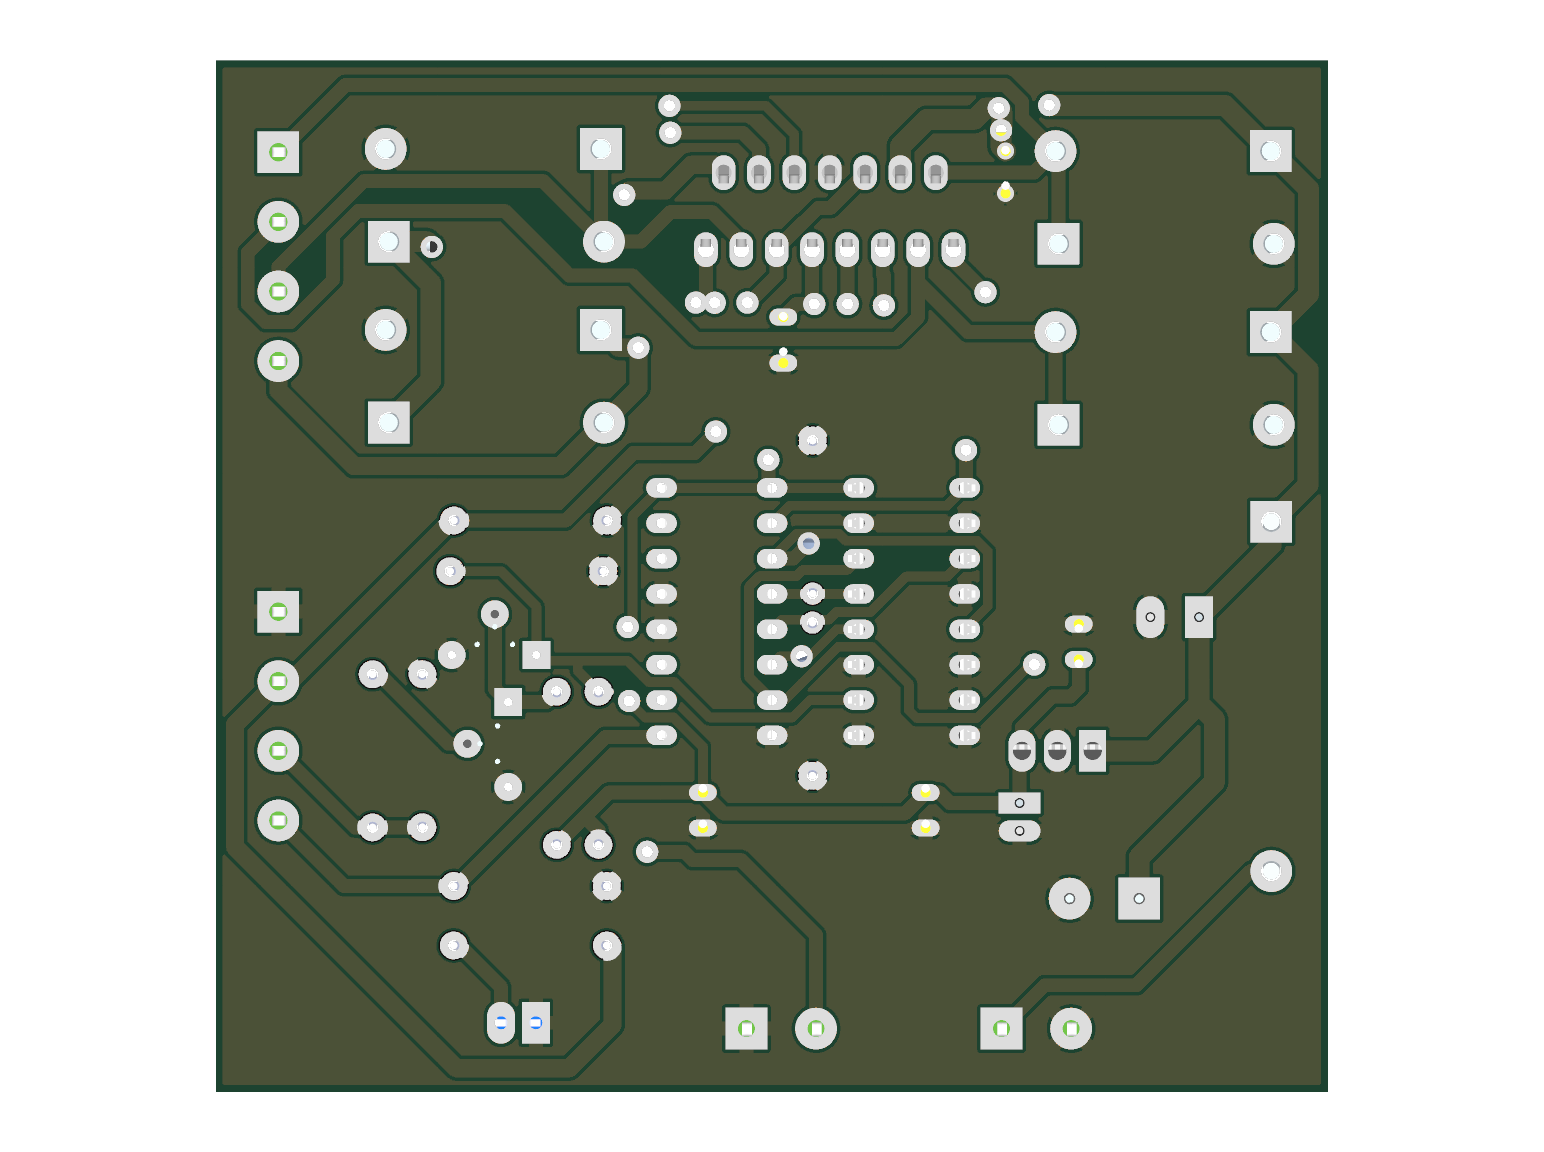
\includegraphics[width=\textwidth]{pcb_bottom.png}
    \caption{Vista inferior con plano de masa y ruteado.}
    \label{fig.ej4:pcb_bottom}
  \end{subfigure}
  \caption{Vistas tridimensionales de la placa \texttt{ctrl\_pap} exportadas desde KiCad.}
  \label{fig.ej4:vistas_pcb}
\end{figure}

En conjunto suma 38 componentes pasantes, 124 pads metalizados y 24 vías entre caras. La tabla~\ref{tab.ej4:bom}
detalla la lista de materiales completa.

\begin{table}[!ht]
  \centering
  \resizebox{\textwidth}{!}{
    \begin{tabular}{|l|c|l|p{6.5cm}|}
      \hline
      \textbf{Designador} & \textbf{Cant.} & \textbf{Valor / Modelo} & \textbf{Función en el circuito} \\ \hline
      \texttt{C1} & 1 & $470\uF$ / $35\V$ electrolítico & Almacenamiento principal de carga en \texttt{VS}. \\ \hline
      \texttt{C2, C3, C4, C7, C8} & 5 & $100\nF$ cerámico &
        Desacople de alta frecuencia en \texttt{VSS} y \texttt{VS}. \\ \hline
      \texttt{C5} & 1 & $100\uF$ / $35\V$ electrolítico & Filtrado auxiliar del bus de potencia \texttt{VS}. \\ \hline
      \texttt{C6} & 1 & $10\uF$ / $35\V$ electrolítico &
        Estabilización de salida \texttt{VSS} en \texttt{IC4}. \\ \hline
      \texttt{D1} & 1 & \texttt{1N5408} ($1000\V$, $3\A$) &
        Protección contra inversión de polaridad en \texttt{J1}. \\ \hline
      \texttt{D2--D9} & 8 & \texttt{1N5822} Schottky ($40\V$, $3\A$) &
        Enclavamiento de transitorios inductivos del motor. \\ \hline
      \texttt{IC1} & 1 & \texttt{L298N} (Multiwatt-15) & Doble puente H de potencia para fases A y B. \\ \hline
      \texttt{IC2} & 1 & \texttt{SN74LS175N} (DIP-16) & Cuádruple biestable D; memoria de estado y salidas. \\ \hline
      \texttt{IC3} & 1 & \texttt{CD4052BF} (DIP-16) & Multiplexor CMOS doble; lógica de próximo estado. \\ \hline
      \texttt{IC4} & 1 & \texttt{LM7805CT} (TO-220) &
        Regulador lineal de $+5\V$ para el bus lógico \texttt{VSS}. \\ \hline
      \texttt{J1, J5} & 2 & Bornera 2 pines ($5\,\unit{\milli\meter}$) &
        Entrada de potencia y salida de retorno de sensado. \\ \hline
      \texttt{J3, J4} & 2 & Bornera 4 pines ($5\,\unit{\milli\meter}$) &
        Entrada de control lógico y salida hacia bobinas. \\ \hline
      \texttt{LED1} & 1 & LED azul $3\,\unit{\milli\meter}$ ($467\,\unit{\nano\meter}$) &
        Indicador luminoso de estado de \texttt{ENABLE}. \\ \hline
      \texttt{Q1, Q2} & 2 & \texttt{BC337} NPN (TO-92) & Etapa adaptadora no inversora de $3.3\V$ a $5\V$. \\ \hline
      \texttt{R3, R11} & 2 & $10\kohm$ ($0.25\,\W$) & Fijación a masa en \texttt{ENABLE} y \texttt{DIR3V3}. \\ \hline
      \texttt{R4} & 1 & Sin montaje (huella axial) & Opción de fijación a masa en \texttt{DIR}, no poblada. \\ \hline
      \texttt{R5} & 1 & $1\kohm$ ($0.25\,\W$) & Terminación a masa en la línea \texttt{STEP}. \\ \hline
      \texttt{R6} & 1 & $470\ohm$ ($0.25\,\W$) & Limitación de corriente para \texttt{LED1}. \\ \hline
      \texttt{R7, R8} & 2 & $6.8\kohm$ ($0.25\,\W$) & Descarga a masa en nodos \texttt{D1} y \texttt{D0}. \\ \hline
      \texttt{R9, R10, R12} & 3 & $4.7\kohm$ ($0.25\,\W$) &
        Polarización de base y carga del adaptador \texttt{Q1}--\texttt{Q2}. \\ \hline
    \end{tabular}
  }
  \caption{Lista de materiales completa de la placa \texttt{ctrl\_pap}.}
  \label{tab.ej4:bom}
\end{table}
